\documentclass[12pt,review,authoryear]{elsarticle}
%\usepackage[numbers]{natbib}
%\usepackage[authoryear]{natbib}
%\usepackage[model1-num-names.bst]{natbib}
\usepackage{hyperref}
%\usepackage[justification=centering]{caption}

\usepackage{float}
\usepackage{subcaption}
\usepackage{caption}
\usepackage[authoryear]{natbib}
\usepackage{url}
\usepackage{etoolbox}% http://ctan.org/pkg/etoolbox
\usepackage{comment}
\usepackage{todonotes}
\usepackage{gensymb}
\usepackage{comment}
\usepackage{gensymb}

\usepackage{enumitem}
\usepackage{amsmath, amsthm, amssymb}
\usepackage{booktabs} % For professional-looking tables
\usepackage{siunitx} % For units formatting
\usepackage{tabularx}
\usepackage{xcolor}
\usepackage{seqsplit}
\usepackage{booktabs}
\usepackage{amsmath}
\usepackage{arydshln}
\usepackage{multirow}
\usepackage{cite}
\usepackage{amsmath}
\usepackage{geometry}
\usepackage{rotating}
\usepackage{enumitem}   
\usepackage{algorithm}
 %\usepackage{algorithmic}
\usepackage{algpseudocode}
\usepackage{amssymb}
\usepackage{amsmath}
\usepackage{graphicx}
\usepackage{algorithm}
\usepackage{cleveref} 
\usepackage{amsmath, amsthm}
\usepackage{courier}
\usepackage{tikz}
\usepackage{enumerate}

\usetikzlibrary{positioning, arrows.meta}

\usepackage{enumitem} % For customized lists

% Define a new theorem style with upright text
\newtheoremstyle{upright}% Name
  {3pt}% Space above
  {3pt}% Space below
  {}% Body font
  {}% Indent amount
  {\bfseries}% Theorem head font
  {.}% Punctuation after theorem head
  { }% Space after theorem head
  {}% Theorem head spec

% Apply the new theorem style
\theoremstyle{upright}
\newtheorem{theorem}{Theorem}


\usepackage{amsmath}
\usepackage{amssymb}
\usepackage{tikz}
\usetikzlibrary{shapes, arrows.meta, positioning}
\usepackage{caption}
\usepackage{cite}
\usepackage{enumitem}
\usetikzlibrary{automata}
\usepackage{pgfplots}
%\AtBeginEnvironment{bmatrix}{\setlength{\arraycolsep}{1pt}}
 %\usepackage{algorithmic}
\usepackage{algpseudocode}
\geometry{a4paper,scale=0.82}
\renewcommand*{\arraystretch}{0.8}
\DeclareSymbolFont{largesymbol}{OMX}{yhex}{m}{n}
\usepackage{appendix}
\DeclareMathAccent{\Widehat}{\mathord}{largesymbol}{"62}
%\usepackage[printonlyused,withpage]{acronym}
%\usepackage{acro}
\def\UrlBreaks{\do\A\do\B\do\C\do\D\do\E\do\F\do\G\do\H\do\I\do\J
\do\K\do\L\do\M\do\N\do\O\do\P\do\Q\do\R\do\S\do\T\do\U\do\V
\do\W\do\X\do\Y\do\Z\do\[\do\\\do\]\do\^\do\_\do\`\do\a\do\b
\do\c\do\d\do\e\do\f\do\g\do\h\do\i\do\j\do\k\do\l\do\m\do\n
\do\o\do\p\do\q\do\r\do\s\do\t\do\u\do\v\do\w\do\x\do\y\do\z
\do\.\do\@\do\\\do\/\do\!\do\_\do\|\do\;\do\>\do\]\do\)\do\,
\do\?\do\'\do+\do\=\do\#} 

%\usepackage[style=alphabetic,maxnames=4,minnames=3,maxbibnames=99]{biblatex}
%\usepackage[style=authoryear]{biblatex}
%\addbibresource{cas-refs.bib}
%%%Author macros
\def\tsc#1{\csdef{#1}{\textsc{\lowercase{#1}}\xspace}}
\tsc{WGM}
\tsc{QE}
\tsc{EP}
\tsc{PMS}
\tsc{BEC}
\tsc{DE}
%%%
\usepackage{amsmath,amsthm,amssymb}

% Define theorem-like environments
\newtheorem{lemma}{Lemma}
%\newtheorem{theorem}{Theorem}
\usepackage{framed} % Framing content
\usepackage{multicol} % Multiple columns environment
%\usepackage{authblk}
\usepackage{nomencl} % Nomenclature package
\usepackage{booktabs}
\usepackage{lineno}
\usepackage{bm}
\makenomenclature
\setlength{\nomitemsep}{-\parskip} % Baseline skip between items
\renewcommand{\nomname}{Abbreviations}
\renewcommand*\nompreamble{\begin{multicols}{2}}
\renewcommand*\nompostamble{\end{multicols}}
\renewcommand{\thefootnote}{*}
\begin{document}
\let\WriteBookmarks\relax
\def\floatpagepagefraction{1}
\def\textpagefraction{.001}

%\begin{frontmatter}
\title{Quantifying Travel Sequence Predictability via a Constrained Vector-Quantized Variational Autoencoder}

%\title [mode = title]{Empirical analysis of electric vehicles' charging patterns: Case study from Shanghai}       


%\author[1,2]{Zhi Li}[orcid=0000-0002-5701-8127]%[type=editor]
                        %auid=000,bioid=1]
                        %role=Researcher,
                      %orcid=0000-0001-7511-2910]

\author[1,2,3]{Zhi Li}%[orcid=0000-0002-5701-8127]
%\author[4]{Wei Ma}
%\author[5]{Monica Menendez}
\author[1,2]{Zhibin Chen\corref{cor1}}
\ead{zc23@nyu.edu.}
\author[4]{Minghui Zhong}
\cortext[cor1]{Corresponding author}

\renewcommand{\algorithmicrequire}{ \textbf{Input:}} 
\renewcommand{\algorithmicensure}{ \textbf{Output:}}  

\affiliation[1]{organization={Shanghai Frontiers Science Center for Data Science, NYU Shanghai},
%addressline={567 West Yangsi Road},
city={Shanghai},
%postcode={200126},
country={China}}

\affiliation[2]{organization={Shanghai Key Laboratory of Urban Design and Urban Science, NYU Shanghai},
%addressline={567 West Yangsi Road},
city={Shanghai},
%postcode={200126},
country={China}}

\affiliation[3]{organization={Department of Civil and Urban Engineering, New York University},
%addressline={6 MetroTech Center},
city={Brooklyn},
%postcode={NY 11201},
country={United States}}



\affiliation[4]{organization={Shanghai Electric Vehicle Public Data Collecting, Monitoring, and Research Center},
%addressline={ 888 Moyunan Road},
city={Shanghai},
%postcode={201805},
country={China}}



\begin{abstract}
A travel sequence is a time-ordered record of travel-related states (e.g., location, speed, and energy consumption rate). Understanding the intrinsic predictability of travel sequences is essential for developing robust and interpretable mobility models. While classical entropy-based methods have been effective for analyzing discrete symbolic sequences, real-world mobility data such as GPS trajectories, driving speed, and battery state are inherently continuous and often form complex, multi-dimensional time series. This disconnect limits the applicability of existing predictability measures in practical transportation settings. In this study, we propose a unified framework that extends discrete-sequence predictability theory to continuous behavioral signals through a novel predictability-distortion framework grounded in rate-distortion theory. Leveraging a Vector-Quantized Variational Autoencoder and augmented Lagrangian optimization, our method estimates the upper bound of behavioral predictability under user-specified reconstruction constraints. Validation on synthetic data confirms the theoretical soundness of the approach. Large-scale experiments using 16 months of operational data from 3,777 electric vehicles in Shanghai further demonstrate its effectiveness: under a 5\% state-of-charge (SOC) error and 2.5 km spatial resolution, the average behavioral predictability reaches 93.98\%, revealing strong regularity in real-world EV usage patterns.
The implementation code and reproducible experiments are publicly available at\url{https://github.com/zhilee2023/Quantifying-the-Predictability-of-Travel-Sequences}





\begin{keyword}
Predictability; Travel Behavior; Vector-Quantized Variational Autoencoder; Electric Vehicle; Information-Theoretic Metrics
\end{keyword}
\end{abstract}


\maketitle

\section{Introduction}

\label{introduction}
%预测在travel behavior的重要性
A travel sequence is a time-ordered record of travel-related states (e.g., location, speed, time,energy consumption rate and mode of travel), capturing how a travel-related condition evolves over successive timestamps. Travel sequence prediction is fundamental to modern mobility systems \citep{chow2018informed}. Accurate forecasting of travel sequence information underpins a broad range of transportation applications, from real-time traffic management and dynamic routing to long-term infrastructure planning and system optimization. For instance, travel time prediction forms the backbone of modern navigation systems, enabling precise route guidance and timely decision-making \citep{chiabaut2021traffic, derrow2021eta}, while public transit arrival time prediction improves service reliability and enhances passenger satisfaction \citep{singh2022review, ricard2022predicting}. Other critical applications include origin-destination demand estimation for ride-hailing platforms to optimize vehicle dispatch and responsiveness \citep{liu2022machine, lin2023deep}, energy demand forecasting for electric vehicles (EVs) to support load balancing and grid-aware charging \citep{ullah2021electric, palaniyappan2024dynamic}, and anticipatory traffic signal control using vehicle trajectory predictions to reduce delays and improve intersection performance \citep{wang2022trajectory, zhu2024multi}.

Despite differences in scale and data requirements, these tasks share a common objective: leveraging patterns in individual and collective mobility to anticipate future behavior and enable smarter transportation systems. To realize this, a wide range of predictive models has been developed, with performance often varying depending on behavioral regularity and task complexity. Regression-based models, such as linear and logistic regression, remain widely used due to their interpretability and computational efficiency, particularly in applications such as travel flow estimation, travel demand prediction, and energy consumption modeling \citep{rajeh2023modeling, kim2020stepwise, de2015energy}. Tree-based ensemble models, such as random forests and gradient boosting machines, demonstrate strong performance in capturing nonlinear interactions and heterogeneous user behavior \citep{chung2019ensemble, shahriar2021prediction}. Bayesian approaches further incorporate probabilistic reasoning and user-specific variation, enabling personalized predictions with uncertainty quantification \citep{chen2023probabilistic, sengupta2024bayesian}. With the proliferation of large-scale time-series and spatial mobility data, deep learning models have become increasingly prominent. These include recurrent architectures (e.g., Long Short-Term Memory networks) \citep{hochreiter1997long, fu2016using}, Transformer-based models for long-range sequence modeling \citep{vaswani2017attention, reza2022multi}, and graph-based models (e.g., Graph Neural Networks) designed to capture relational structures in road networks \citep{li2017diffusion, zhao2019t}. More recently, large language models (LLMs) adapted for mobility tasks have shown strong generalization across diverse prediction objectives \citep{mo2023large,wang2023would}.

While recent advances in model architectures have significantly improved predictive accuracy, they predominantly address the how of prediction, focusing on algorithmic enhancements tailored to specific tasks.  In contrast, a complementary and increasingly prominent research direction asks a more fundamental question: what is the theoretical upper limit of predictability for a given behavior, regardless of the predictive model used? This paradigm introduces the notion of intrinsic predictability, which quantifies the underlying regularity or randomness embedded in travel sequences. Pioneering work by \citet{song2010limits} lays the theoretical foundation by proposing an information-theoretic framework to estimate the upper bound of human mobility predictability using entropy-based metrics derived from anonymized mobile phone data. Their analysis demonstrated that, despite considerable variability in transportation mode choices, individual mobility patterns exhibit remarkably high regularity, with an average potential predictability of approximately 93\%.  Building on this framework, subsequent studies have applied similar entropy-based methodologies to a variety of transportation contexts. For instance, \citet{li2014limits} examined the predictability limits of urban vehicular mobility using large-scale vehicle trajectory datasets, and reported that approximately 78-99\% of vehicle locations and over 70\% of dwell times are theoretically predictable. \citet{goulet2017measuring} further extended this line of inquiry by analyzing the regularity of individual travel behavior using a large-scale dataset of transit smart card transactions from London. They modeled daily travel as sequences of discrete events and estimated entropy rates to capture the contribution of both event frequency and temporal order. Further, \citet{alipour2019you} investigated mobility predictability in a campus-scale wireless network, demonstrating that user behavior, shaped by device type, affects movement predictability across spatiotemporal scales.

Although most studies on mobility predictability rely on discrete sequences, many traffic-related time series (e.g., travel time and speed) are inherently continuous. To bridge this gap, recent research has extended classical frameworks to accommodate continuous signals. For instance, \citet{li2019travel} proposed a revised Lempel-Ziv (LZ) entropy measure tailored to continuous travel time data, enabling distribution-free estimation of sequential regularity beyond conventional reliability metrics. Further, \citet{li2022estimate} advanced this line of inquiry by introducing an information-theoretic framework that leverages conditional differential entropy and a continuous form of Fano’s theorem to establish theoretical lower bounds on predictability. %These efforts mark a significant shift from discrete-symbol-based predictability analysis to rigorous, entropy-driven evaluations of continuous traffic dynamics.

Despite recent progress, important gaps remain in quantifying and comparing travel behavior predictability, particularly for multi-dimensional and continuous signals:
\begin{enumerate}[(1)]
\item Most existing studies on predictability focus on bounding the performance of forecasting models, for example estimating theoretical lower or upper bounds for traffic variables such as speed or travel time using revised LZ entropy or a continuous form of Fano’s theorem \citep{li2022estimate,li2019travel}.
However, we still lack a coherent, generalizable theory that carries discrete sequence-based predictability to continuous behavioral signals, with explicit, comparable metrics at the whole-sequence level rather than only next-step bounds.

\item Real-world travel behavior typically involves multiple interdependent variables, such as speed, location, and energy usage, that evolve jointly over time. While most prior research focuses on single-variable sequences \citep{song2010limits,li2019travel,li2022estimate}, methods for evaluating the overall predictability of multi-dimensional, temporally correlated signals are still lacking. To the best of our knowledge, no unified framework has been proposed to systematically quantify the joint predictability embedded in these complex behavioral dynamics.

\item Even when predictability can be estimated at the individual level, few methods allow for standardized comparison of behavioral regularity across users. Without scale-consistent and interpretable metrics, it remains difficult to quantify inter-individual differences in sequence predictability, limiting the practical use of such measures in behavior modeling, personalization, and equity-aware decision-making.
\end{enumerate}


To address the above challenges, we propose a quantization-based framework that leverages Vector Quantized Variational Autoencoders (VQ-VAE) \citep{van2017neural} to compress continuous mobility signals into a discrete latent space. This transformation enables the application of entropy-based methods traditionally designed for symbolic sequences. Given a fixed reconstruction loss that preserves task-relevant information, we compute the maximum achievable predictability of the resulting discrete representation using established information-theoretic estimators. This approach allows for a unified treatment of continuous, multi-dimensional travel sequences and provides a scalable basis for comparing predictability across individuals.


Our contributions are twofold:
\begin{enumerate}[(1)]
    \item We extend discrete-sequence predictability theory to continuous signals by introducing a framework for mobility analysis inspired by rate-distortion theory. Specifically, we formalize the predictability-distortion tradeoff as the maximum achievable predictability of a sequence under a given reconstruction-loss constraint. This formulation bridges the gap between information-theoretic predictability measures and continuous behavioral data.
    
    \item We develop a practical solution by integrating this framework with VQ-VAE , which compress continuous multi-dimensional travel sequences into discrete representations while controlling distortion. This enables the systematic estimation and comparison of individual-level predictability, offering new insights into behavioral regularity across heterogeneous users.
\end{enumerate}

The remainder of this paper is organized as follows. Section \ref{Methodology} introduces our methodology: we begin by reviewing discrete predictability theory, then extend it to continuous signals via a predictability-distortion framework, and finally present a VQ-VAE-based optimization approach using augmented Lagrangian methods. Section \ref{experiment} provides experimental validation through two studies: a synthetic sequence with known rate-distortion behavior to verify theoretical consistency, and a large-scale real-world application using 16 months of 10-minute interval data from 3,777 battery electric vehicles (BEVs) to evaluate individual predictability and compare it with baseline forecasting models. Section \ref{conclusion} concludes the paper.








\section{Methodology}
\label{Methodology}

\subsection{Predictability of a discrete traveling signal process}
\noindent
Consider a discrete traveling random process 
$\{Z_t\}_{t=1}^L$ 
taking values in a finite set $\mathcal{Z}$ of cardinality $N = |\mathcal{Z}|$. Assume that $\{Z_t\}$ is a stationary process. According to \citet{song2010limits}, the following relationship holds:

\begin{equation}
H\left(Z_n \mid Z_1, Z_2, \dots, Z_{n-1}\right) \leq H^{\mathrm{unc}} \leq H^{\mathrm{rand}},
\end{equation}

\noindent where:

\begin{enumerate}[(1)]
  \item \textbf{Conditional Entropy} $H\left(Z_n \mid Z_1, Z_2, \dots, Z_{n-1}\right)$:  
  This represents the entropy of the next travel signal $Z_n$ given the historical travel signals:  \[Z_1, Z_2, \dots, Z_{n-1}.\]
  
  \item \textbf{Temporal-Uncorrelated Entropy} $H^{\mathrm{unc}}$:  
  This entropy measure focuses on the heterogeneity of visitation frequencies while ignoring temporal correlations:
  \[
    H^{\mathrm{unc}} = -\sum_{z \in \mathcal{Z}} 
    p(z)\,\log_2 p(z),
  \]
 where $p(z) = p(Z_t)$ for all $t$ due to the stationarity property. Since the distribution is time-invariant, the empirical probability of observing state $z$ in $\mathcal{Z}$ can be reliably estimated from a sufficiently long observed sequence.
  
  \item \textbf{Random Entropy} $H^{\mathrm{rand}}$:  
  This assumes that each state in $\mathcal{Z}$ is visited with equal probability, representing maximal disorder:
  \[
    H^{\mathrm{rand}} = \log_2 \lvert \mathcal{Z} \rvert.
  \]
\end{enumerate}
In essence, the inequality indicates that the entropy of random destination selection represents the upper bound of uncertainty, which is reduced when accounting for visitation frequency, and further minimized when temporal dependencies are incorporated into the prediction.

Since the sequence \(H\left(Z_n \mid Z_1, Z_2, \dots, Z_{n-1}\right) \) is monotonically decreasing in $n$ and bounded below by zero according to \citet{cover1999elements}, it must converge to a finite limit. Consequently,
$$
\lim_{n\to\infty} H\!\bigl(Z_n \mid Z_1,\dots,Z_{n-1}\bigr) \leq H\left(Z_n \mid Z_1, \ldots, Z_{n-1}\right).
$$

For a stationary stochastic process, this limit coincides with the entropy rate \citep{cover1999elements}:

$$
H_{\text {rate }}:=\lim _{n \rightarrow \infty} \frac{H\left(Z_1, \ldots, Z_n\right)}{n}=\lim _{n \rightarrow \infty} H\left(Z_n \mid Z_1, \ldots, Z_{n-1}\right),
$$
Putting these facts together yields the chain of inequalities:

\begin{align}
      H_{\mathrm{rate}} = \lim_{n\to\infty} H\!\bigl(Z_n \mid Z_1,\dots,Z_{n-1}\bigr)
  \le H\!\bigl(Z_n \mid Z_1,\dots,Z_{n-1}\bigr)
       \le H^{\mathrm{unc}}
       \le H^{\mathrm{rand}}.
\label{eq:song}
\end{align}

According to Fano's inequality \citep{cover1999elements}, the conditional entropy, $H\bigl(Z_n \mid Z_1,\allowbreak\dots,\allowbreak Z_{n-1}\bigr)$, provides a lower bound on the probability of error, defined by \( P_e = P(Z_n \neq \hat{Z}_n) \), in predicting \( Z_n \) given the historical signals \( Z_1, Z_2, \dots, Z_{n-1} \). Here, $\hat{Z}_n$ denotes the predicted value of $Z_n$ based on the optimal estimator that utilizes the past observations $Z_1^{n-1}=\left(Z_1, Z_2, \ldots, Z_{n-1}\right)$.  Specifically, Fano's inequality relates the conditional entropy to the error probability \( P_e \) as follows:
    
\begin{equation}
    H\left(Z_n \mid Z_1, \dots, Z_{n-1}\right) \leq H_b(P_e) + P_e \log_2 \left(|\mathcal{Z}| - 1\right),
    \label{eq:finoeq}
\end{equation}
where \( H_b(P_e) = -P_e \log_2 P_e - (1 - P_e) \log_2 (1 - P_e) \) is the binary entropy function. This implies that a lower conditional entropy corresponds to a lower error probability in predicting \( Z_n \). Let \( f_e(P_e) = H_b(P_e) + P_e \log_2 \left(|\mathcal{Z}| - 1\right) \), then $f_e\left(P_e\right) \geq H_{\text {rate }}$ by Eqs. (\ref{eq:song}) and (\ref{eq:finoeq}). \citet{song2010limits} showed that for $P_e \in \left[0, 1 - \frac{1}{|\mathcal{Z}|}\right]$, the function $f_e(P_e)$ is monotonically increasing, taking values within the range $[0, \log_2 |\mathcal{Z}|]$. Therefore, when $f_e\left(P_e\right)=H_{\text {rate }}$, the prediction error probability $P_e$ attains its minimum value $P_e^{\min }$, yielding the maximum achievable predictability $\Pi^{\max }=1-P_e^{\min }$. Thus, the predictability of the travel sequence can be derived using the entropy rate of the sequence and the equation \( f_e(1-\Pi^{\mathrm{max}}) = H_{\mathrm{rate}} \). Typically, the entropy rate of discrete sequences can be estimated using methods such as the Lempel-Ziv (LZ) algorithm, context-weighted tree (CTW) approaches, and other advanced techniques.

\subsection{From discrete-signal to continuous-signal predictability theory}
However, Song's theory does not account for the effects of discretization. Clearly, varying degrees of discretization lead to differences in the maximum predictability of signals. For example, in the case of GPS signals, the scale of discretization significantly impacts their predictability. Simply put, partitioning a city into 10-kilometer square regions results in noticeably higher predictability compared to dividing it into 500-meter square grids. Even under the same spatial resolution, the manner in which the signal is discretized can greatly affect the resulting predictability. As illustrated in Figure~\ref{fig:hexgonplot}, consider two spatial points A and B. In the left panel, A and B are located near the boundary between two hexagonal regions, Zone 1 and Zone 2. If a traveler randomly switches between these two locations, the sequence alternates between Zone 1 and Zone 2, yielding a predictability of 50\%. In contrast, the right panel shows an alternative discretization scheme with the same hexagonal resolution, where both A and B are assigned to Zone 1. In this case, the resulting sequence becomes homogeneous, leading to a predictability of 100\%. Therefore, determining how to discretize continuous travel signals, such as GPS trajectories, at a given scale is key to extending predictability analysis from discrete to continuous domains. In addition, discretization will inevitably introduce information loss; for example, converting continuous GPS coordinates into spatial grids sacrifices precise locational details. As a result, both the scale and manner of discretization affect the maximum achievable predictability for each individual. To enable fair and comparable predictability estimation across users, such comparisons must be conditioned on a consistent level of information loss. To this end, we adopt the framework of rate-distortion theory from information theory and develop a predictability-distortion theory, which characterizes the upper bound of behavioral predictability under a given reconstruction distortion. 
\begin{figure}[htbp!]
    \centering
    \includegraphics[width=0.85\linewidth]{hexgonplot.pdf}
    \caption{Two discretization schemes with identical resolution}
    \label{fig:hexgonplot}
\end{figure}

\subsubsection{Rate-distortion theory}

Let $X=\left\{X_t\right\}_{t=1}^{\infty}$ be a stationary ergodic source with each $X_t \in \mathcal{X} \subseteq \mathbb{R}^q$. For any positive integer $n$, we define the block of source symbols as $X^n=\left(X_1, X_2, \ldots, X_n\right) \in \mathcal{X}^n$. The encoder is a mapping $\mathcal{F}: \mathcal{X}^n \rightarrow \mathcal{Z}^n$, where $\mathcal{Z}$ is a finite (discrete) alphabet, so that $Z^n =\left(Z_1, Z_2, \ldots, Z_n\right)$ = $\mathcal{F}\left(X^n\right) \in \mathcal{Z}^n$. A decoder $\mathcal{G}: \mathcal{Z}^n \rightarrow \hat{\mathcal{X}}^n \subseteq \mathbb{R}^q$ then reconstructs the signal, yielding $\hat{X}^n=$ $\mathcal{G}\left(Z^n\right)$. Information loss is quantified by a \emph{single-letter} distortion  
\(d:\mathcal{X}\times\hat{\mathcal{X}}\to\mathbb{R}_{\ge0}\)  
. For instance, the squared error \(d(x,\hat x)=\lVert x-\hat x\rVert^{2}\).  
Its per-letter block extension is: 
\[
d_{n}(x^{n},\hat x^{n})
=\frac{1}{n}\sum_{t=1}^{n} d(x_{t},\hat x_{t}).
\]
The encoder-decoder pair \((\mathcal{F},\mathcal{G})\) must satisfy the
average-distortion constraint:
\[
\mathbb{E}\!\left[d_{n}\!\bigl(X^{n},\hat X^{n}\bigr)\right]\;\le\;D.
\]
where \(D>0\) is the prescribed tolerance.

Accordingly, this Encoder-Decoder framework is illustrated in Figure \ref{fig:encoder_decoder_architecture}.

\begin{figure}[ht]
    \centering
    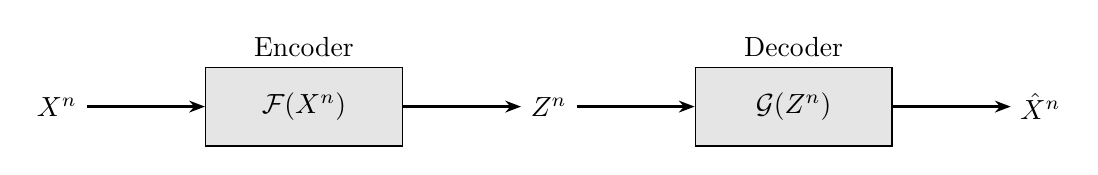
\begin{tikzpicture}[
        node distance=0.01cm and 1.5cm,
        box/.style={rectangle, draw, minimum width=2.5cm, minimum height=1cm, fill=gray!20, align=center},
        arrow/.style={-{Stealth[length=2mm]}, thick, font=\small}
    ]

        % Define nodes
        \node (X)  {$X^n$};
        \node (encoder) [box, right=of X] {$\mathcal{F}(X^n)$};
        \node (z) [ right=of encoder] {$Z^{n}$};
        \node (decoder) [box, right=of z] {$\mathcal{G}(Z^{n})$};
        \node (xhat) [right=of decoder] {$\hat{X}^n$};

        \node (encoder_label) [above=of encoder] {Encoder};
        \node (decoder_label) [above=of decoder] {Decoder};
    
        % Draw arrows with labels
        \draw [arrow] (X) -- node[above]{} (encoder);
        \draw [arrow] (encoder) -- node[above]{} (z);
        \draw [arrow] (z) -- node[above]{} (decoder);
        \draw [arrow] (decoder) -- node[above]{} (xhat);
    \end{tikzpicture}
    \caption{Encoder-Decoder architecture}
    \label{fig:encoder_decoder_architecture}
\end{figure}

A fundamental question in information and communication theory is: What is the minimum transmission rate or number of storage bits required for the compressed signal $Z^n$ to ensure that the distortion rate during transmission or storage remains within allowable distortion? To address this, \citet{gallager1968information} proposed the rate-distortion theory to general stationary source.


\begin{theorem}[Gallager, 1968]\label{theorem Gallager}
%\textbf{Rate-Distortion Function for Non-I.I.D. Ergodic Sources}

For a stationary ergodic  source \( X=\{X_t\}_{t=1}^{ \infty} \), the lower bound for the transmission bit-rate given the maximum allowable distortion $D$ is: 

\begin{align*}
    R(D) :=& \inf_{n} \min_{p(\hat{X}^n \mid X^n)} \frac{1}{n} I(X^n; \hat{X}^n):=\inf_{n} R_n(D)\\
    &=\lim_{n \to \infty} \min_{p(\hat{X}^n \mid X^n)} \frac{1}{n} I(X^n; \hat{X}^n) 
     \\
     \text{s.t.}\\
    %&\frac{1}{n} \sum_{t=1}^n \mathbb{E}\left[d \left(X_t, \hat{X}_t\right)\right] \leq D, \\
    & \mathbb{E}\!\left[d_{n}\!\bigl(X^{n},\hat X^{n}\bigr)\right]\;\le\;D,%\mathbb{E}\left[d\left(X^n_t, \hat{X}^n_t\right)\right] \leq D
    %\intertext{subject to:}
    %&\frac{1}{m} \sum_{t=1}^m \mathbb{E}\left[d(X_t, \hat{X}_t)\right] \leq D, \label{eq:distConstraint}
\end{align*}
where the components are defined as follows:
\begin{itemize}
    \item \( p(\hat{X}^n \mid X^n) \) is the conditional probability distribution that maps the source sequence \( X^n \) to the reconstructed sequence \( \hat{X}^n \).
    \item \( I(X^n; \hat{X}^n) \) denotes the mutual information between the source sequence \( X^n \) and the reconstructed sequence \( \hat{X}^n \), which quantifies the amount of information one random variable contains about another. 

\end{itemize}
\end{theorem}
According to the aforementioned rate-distortion theory, the minimal mutual information exists under the distortion constraint \( D \). Furthermore, as \( n \) increases, \( R_n(D) \) converges to \( R(D) \), representing this minimal mutual information. Additionally, for different values of \( D \), we can determine the minimal transmission rate or the optimal storage rate  \( R(D) \). Therefore, for traveling signals, based on the aforementioned theory, we propose that under different discretizations, the discretized symbol sequence \( Z^n \) exhibits maximal predictability, referred to as the predictability-distortion theory.










\subsubsection{Predictability-distortion theory}
To establish the connection between $Z^n$ and mutual information, an intuitive approach is to consider that when $Z^n$ is decoded into $\hat{X}^n$, one may define a mapping $g^{\prime}$, if it exists,that reconstructs $Z^n$ from the reconstructed information $\hat{X}^n$. Thus, when $Z^n$ and $\hat{X}^n$ are in a one-to-one correspondence, we have the following lemma:
\newline
\begin{lemma}\label{thm:mutual_information_equality}
Consider a continuous source $\left\{X_t\right\}_{t=1}^n$ and an encoder $\mathcal{F}: \mathcal{X}^n \rightarrow \mathcal{Z}^n$ that maps the source to a discrete alphabet $\mathcal{Z}^n$, with $Z^n = f\left(X^n\right)$. A decoder $\mathcal{G}: \mathcal{Z}^n \rightarrow \mathcal{X}^n$ maps $Z^n$ back to $\hat{X}^n = \mathcal{G}\left(Z^n\right)$. The condition $H\left(Z^n \mid \hat{X}^n\right) = 0$ is both necessary and sufficient for $H\left( Z^n\right) = I\left(X^n; \hat{X}^n\right)$.

%(which may form a Markov chain or, more generally, any arbitrary process) and two mappings $g: \mathcal{X}^n \to \mathcal{Z}^m 
\end{lemma}


\begin{proof}
See \ref{Proof of Lemma 1}.
\end{proof}
Thus, by the lemma, it follows that, in order to jointly account for the entropy rate of the latent space and the mutual information $I\left(X^n ; \hat{X}^n\right)$, it is imperative that:
\[
H\left(Z^n \mid \hat{X}^n\right) = 0.
\]
Therefore, we can transform the problem $R_n(D)$ in Theorem \ref{theorem Gallager} into the following problem:
%因此定理 \ref{theorem Gallager}可以被重新定义为以下的问题：
$$
R_n(D)=\min _{\mathcal{G}, \mathcal{F}} \frac{1}{n} H\left(Z^n\right) \quad \text{s.t.} \quad \mathbb{E}\left[d_n\left(X^n, \hat{X}^n\right)\right] \leq D, H\left(Z^n \mid \hat{X}^n\right)=0.
$$
%进一步的，当我我们限制Z^n使得,Z^n保持statinary，egodic时候，我们有以下的定理：
This formulation seeks an encoder-decoder pair \((\mathcal{F}, \mathcal{G})\) that minimizes the average joint entropy of the latent representation, subject to a distortion constraint and perfect decodability. 

Based on Theorem \ref{theorem Gallager} and Lemma \ref{thm:mutual_information_equality},we propose the following theorem:


\begin{theorem}[Predictability-distortion theory]\label{thm:PD}
Let \(X = \{X_t\}_{t=1}^{\infty}\) be a stationary ergodic source over \(\mathcal{X} \subseteq \mathbb{R}^q\).  
Consider an encoder \(\mathcal{F}: \mathcal{X}^n \rightarrow \mathcal{Z}^n\), where \(Z^n = \mathcal{F}(X^n)\),  
and a decoder \(\mathcal{G}: \mathcal{Z}^n \rightarrow \hat{\mathcal{X}}^n\), where \(\hat{X}^n = \mathcal{G}(Z^n)\). Then the maximum achievable predictability $\Pi$ of the latent representation under distortion constraint \(D\) is given by:
\[
\Pi(D) = 1 - P_e^{\min}(D), \quad \text{where} \quad f_e\left(P_e^{\min }(D)\right)=R(D):=\inf _{n} R_n(D),
\]
where

\[
f_e(p) = H_b(p) + p \log_2(|\mathcal{Z}| - 1), \quad H_b(p) = -p \log_2 p - (1 - p) \log_2 (1 - p),
\]
and
\[
R(D) = \lim_{n \to \infty} R_n(D), \quad \text{s.t.} \quad \mathbb{E}\left[d_n\left(X^n, \hat{X}^n\right)\right] \leq D, H\left(Z^n \mid \hat{X}^n\right)=0.
\]

\end{theorem}

The proof of Theorem~\ref{thm:PD} is intuitive: once the minimum achievable average entropy rate $\inf_n R_n(D)$ in the latent space under the given constraints is established, the maximum predictability can be directly derived based on the theoretical framework proposed by \citet{song2010limits}.

To handle the distortion constraint and the perfect reconstruction constraint, we introduce Lagrange multipliers \(\beta \geq 0\) and \(\lambda \in \mathbb{R}\), respectively. The corresponding Lagrangian becomes:
\begin{equation}
\label{lagrangian}
    \mathcal{L}(\mathcal{F}, \mathcal{G}; \mu, \lambda) = \frac{1}{n} H(Z^n) + \mu\left( \mathbb{E}[d_n(X^n, \hat{X}^n)] - D \right) + \lambda H(Z^n \mid \hat{X}^n),
\end{equation}
Here, the first term represents the coding rate (average entropy), the second enforces the distortion constraint, and the third enforces the perfect decodability. 
%If the constraint \(H(Z^n \mid \hat{X}^n) = 0\) is treated as hard, one can consider taking \(\lambda \to \infty\), or alternatively, retain it explicitly. The resulting optimization becomes
We solve the above optimization problem by combining the augmented Lagrangian method with the VQ-VAE framework.
\subsection{Entropy-constrained VQ-VAE via augmented Lagrangian optimization}

Let each training example be a length-\(n\) block \(X^n = (X_1, X_2, \dots, X_n)\in\mathcal{X}^n\).  The encoder \(\mathcal{F}\) maps:
\[
X^n \;\mapsto\; Z^n \;=\; \bigl(Z_1, Z_2, \dots, Z_n\bigr)\;\in\;\mathcal{Z}^n,
\]
where \(\mathcal{Z}=\{1,\dots,K\}\) is a finite alphabet of size \(K\).  Concretely, for each time index \(t=1,\dots,n\), the encoder first produces a continuous embedding
\[
\mathbf{z}_e\bigl(X_t\bigr)\;\in\;\mathbb{R}^q,
\]
then quantizes it via a shared codebook \(\{\mathbf{e}_j\}_{j=1}^K\subset\mathbb{R}^q\):
\[
k_t^*
\;=\;
\arg\min_{j=1,\dots,K}\;\bigl\lVert \mathbf{z}_e(X_t) - \mathbf{e}_j \bigr\rVert_2,
\qquad
Z_t = k_t^*,
\qquad
\mathbf{z}_q(X_t) = \mathbf{e}_{\,k_t^*}.
\]
Collecting over \(t=1,\dots,n\) yields
\[
Z^n = \bigl(k_1^*,\,k_2^*,\,\dots,\,k_n^*\bigr),
\quad
\hat{\mathbf{Z}}^n = \bigl(\mathbf{z}_q(X_1),\,\mathbf{z}_q(X_2),\,\dots,\,\mathbf{z}_q(X_n)\bigr).
\]
The decoder \(\mathcal{G}\) then reconstructs
\[
\hat{X}^n 
\;=\; 
\bigl(\hat{X}_1,\hat{X}_2,\dots,\hat{X}_n\bigr)
\;=\; 
\mathcal{G}\bigl(\hat{\mathbf{Z}}^n\bigr).
\]
Define the per‐block reconstruction loss as
\[
\mathcal{L}_{\mathrm{rec}}(X^n,\hat{X}^n)
\;=\;
\frac{1}{n}\sum_{t=1}^n \bigl\lVert X_t - \hat{X}_t \bigr\rVert_2^2.
\]
Here, we use the mean squared error as the distortion measure:
\[
d_n\bigl(X^n,\hat{X}^n\bigr)
\;=\;
\frac{1}{n}\sum_{t=1}^n \bigl\lVert X_t - \hat{X}_t \bigr\rVert_2^2.
\]
The standard VQ-VAE loss includes reconstruction, codebook loss, and encoder commitment losses:

\begin{align}
\mathcal{L}_{\mathrm{VQ\text{-}VAE}}(X^n)
= &\ \underbrace{\mathcal{L}_{\mathrm{rec}}(X^n,\hat{X}^n)}_{\text{Reconstruction Loss}} 
+ \underbrace{\frac{1}{n}\sum_{t=1}^n \left\lVert \mathrm{sg}[\mathbf{z}_e(X_t)] - \mathbf{e}_{\,k_t^*} \right\rVert_2^2}_{\text{Codebook Loss}} \notag \\
& + \underbrace{\frac{\beta}{n}\sum_{t=1}^n \left\lVert \mathbf{z}_e(X_t) - \mathrm{sg}[\mathbf{e}_{\,k_t^*}] \right\rVert_2^2}_{\text{Commitment Loss}}.
\end{align}


\noindent where \(\mathrm{sg}[\cdot]\) denotes “stop gradient” and \(\beta>0\) is a constant. We denote \(\mathcal{L}_{\mathrm{VQ}}\) as the sum of the codebook and commitment losses.  Hence, the full VQ-VAE loss can be written as:
\[
\mathcal{L}_{\mathrm{VQ\text{-}VAE}}(X^n)
=
\mathcal{L}_{\mathrm{rec}}
\;+\;\mathcal{L}_{\mathrm{VQ}}.
\]
To approximate the Lagrangian
\[
\mathcal{L}(\mathcal{F},\mathcal{G};\,\mu,\lambda)
=\frac{1}{n}H(Z^n)
\;+\;
\mu\Bigl(\mathbb{E}\bigl[d_n(X^n,\hat{X}^n)\bigr]-D\Bigr)
\;+\;
\lambda\,H\bigl(Z^n\mid\hat{X}^n\bigr),
\]
we add two differentiable penalties for the single block \(X^n\).

\paragraph{1. Entropy penalty $\mathcal{L}_{\mathrm{entropy}}(Z^n)$}
For each \(t=1,\dots,n\) and \(j=1,\dots,K\), define
\[
q_{t,j} \;=\; \,\bigl\lVert \mathbf{z}_e(X_t) - \mathbf{e}_j\bigr\rVert_2^2.
\]
At temperature \(\tau>0\), we follow the technique proposed by \citet{agustsson2017soft} to compute a soft assignment, thereby making the entropy term differentiable:

\[
\tilde{z}_{t,j}
\;=\;
\frac{\exp\bigl(q_{t,j}/\tau\bigr)}
{\displaystyle \sum_{m=1}^K \exp\bigl(q_{t,m}/\tau\bigr)},
\qquad
t=1,\dots,n,\;j=1,\dots,K.
\]
Define the hard assignment index
\[
k_t \;=\; \arg\max_{1\le j\le K}\;q_{t,j},
\]
so that in the limit \(\tau\to 0\), \(\tilde{z}_{t,\cdot}\) becomes the one‐hot vector for \(k_t\).  We form the true marginal
\[
p_j \;=\; \frac{1}{n}\sum_{t=1}^n \mathbf{1}\{\,k_t = j\,\},
\qquad
j=1,\dots,K,
\]
which is the frequency of codeword \(j\) in $\mathcal{Z}$.  The entropy penalty for the block \(X^n\) is then
\[
\mathcal{L}_{\mathrm{entropy}}(Z^n)
=\frac{1}{n}H(Z^n)= -\sum_{j=1}^K p_j \,\log p_j.
\]
In practice, we approximate \(\{p_j\}\) by the soft marginals
\(\bar{p}_j = \frac{1}{n}\sum_{t=1}^n \tilde{z}_{t,j}\), so that
\[
\mathcal{L}_{\mathrm{entropy}}(Z^n)
\approx
-\sum_{j=1}^K \bar{p}_j \,\log \bar{p}_j.
\;%\approx\;-\sum_{j=1}^K \left(\frac{1}{n}\sum_{t=1}^n \tilde{z}_{t,j}\right)\,\log \left(\frac{1}{n}\sum_{t=1}^n \tilde{z}_{t,j}\right).
\]


\paragraph{2. Decodability penalty \(\mathcal{L}_{\mathrm{dec}}(\hat{X}^n)\)}  
Introduce a classifier \(\psi:\hat{\mathcal{X}}^n\to\mathbb{R}^{n\times K}\).  Given \(\hat{X}^n\), for each \(t\) it outputs logits \(\psi(\hat{X}^n)_{t}\in\mathbb{R}^K\).  Denote the true code index 
\[
k_t^* \;=\; \arg\min_{1\le j\le K}\;\bigl\lVert \mathbf{z}_e(X_t) - \mathbf{e}_j\bigr\rVert_2.
\]
Then
\[
\mathcal{L}_{\mathrm{dec}}(\hat{X}^n)
=\frac{1}{n}\sum_{t=1}^n 
\Bigl(-\log\,\mathrm{softmax}\! \bigl(\psi(\hat{X}^n)_{t}\bigr)_{\,k_t^*}\Bigr),
\]
where \(\mathrm{softmax}(\cdot)_{\,k_t^*}\) denotes the predicted probability corresponding to the true label \(k_t^*\).  $\mathcal{L}_{\mathrm{dec}}(\hat{X}^n)$ enforces \(H(Z^n \mid \hat{X}^n)\approx 0\), since the reconstructed signal $\hat{X}^n$ is decoded from codebook entries and therefore deterministically reveals the corresponding latent sequence $Z^n$, resulting in near-zero conditional entropy.

%\paragraph{3. Total loss $\mathcal{L}_{\text{total}}(\mathcal{F},\mathcal{G},\psi;\,\mu,\lambda)$}
Based on the Lagrangian form in Eq.(\ref{lagrangian}), our total loss is defined as follows:
\[
\mathcal{L}_{\mathrm{total}}(X^n)
= \mathcal{L}_{\mathrm{entropy}} + \mu (\mathcal{L}_{\mathrm{rec}}-D + \mathcal{L}_{\mathrm{VQ}}) 
\;+\;\lambda\,\mathcal{L}_{\mathrm{dec}}.
\]
This ensures that \(\mathcal{L}_{\mathrm{total}}(X^n)\) approximates
\[
\frac{1}{n}H(Z^n)
\;+\;
\mu\Bigl(\mathbb{E}\bigl[d_n(X^n,\hat{X}^n)\bigr]-D\Bigr)
\;+\;
\lambda\,H\bigl(Z^n\mid \hat{X}^n\bigr),
\]
while remaining end-to-end differentiable. In summary, our model architecture and is shown in Figure \ref{Network architecture and loss computation pipeline}.

\begin{figure}
    \centering
    \includegraphics[width=1\linewidth]{arch.pdf}
    \caption{Network architecture and loss computation pipeline}
    \label{Network architecture and loss computation pipeline}
\end{figure}



%\paragraph{4. Augmented Lagrangian Optimization}  


To enforce $ \mathcal{L}_{\mathrm{rec}} \leq D$ and $\mathcal{L}_{\mathrm{dec}}=0$, we further adopt the augmented Lagrangian method (ALM). Compared to a pure penalty approach, ALM offers two main benefits:
\begin{enumerate}[(1)]
    \item \textbf{More stable constraint handling:} Combining a moderate quadratic penalty with a Lagrange multiplier avoids the need for excessively large penalties, preventing gradient vanishing or explosion.
    \item \textbf{Faster constraint satisfaction:} Multiplier updates steer the solution toward feasibility even when the penalty term is small, accelerating convergence.
\end{enumerate}

Concretely, let
\[
g_1^+(X^n,\hat{X}^n)
= \max\bigl\{\,\mathcal{L}_{\mathrm{rec}} - D,\;0\bigr\},
\qquad
g_2(X^n,\hat{X}^n)
= \mathcal{L}_{\mathrm{dec}}(\hat{X}^n).
\]  
The augmented Lagrangian is thus
\[
\mathcal{L}_{\mathrm{ALM}}
=
\mathcal{L}_{\mathrm{entropy}}
\;+\;
\mu\,\bigl(g_1^+ + \mathcal{L}_{\mathrm{VQ}}\bigr)
\;+\;
\frac{\rho_1}{2}\,\bigl[g_1^+\bigr]^2
\;+\;
\lambda\,g_2
\;+\;
\frac{\rho_2}{2}\,\bigl[g_2\bigr]^2,
\]

We minimize \(\mathcal{L}_{\mathrm{ALM}}\) over the network parameters \(\{\phi,\theta,\mathbf{e}_j,\psi\}\) (using straight‐through for quantization), then update
\[
\mu \;\leftarrow\; \mu \;+\; \rho_1\,g_1^+,
\qquad
\lambda \;\leftarrow\; \lambda \;+\; \rho_2\,g_2.
\]
If \(g_1^+\) or \(g_2\) remains large, we increase \(\rho_1\) or \(\rho_2\) at the end of each epoch.  This enforces \(\mathbb{E}[d_n]\le D\) and \(H(Z^n\mid\hat{X}^n)=0\) more stably than using a pure penalty method, avoids overly large penalties, and preserves end-to-end differentiability in the VQ-VAE. The full pseudo code of the proposed algorithm is presented in Algorithm \ref{Entropy-constrained VQ-VAE via augmented Lagrangian optimization}.


\begin{algorithm}[t!]
\caption{Entropy-constrained VQ-VAE via augmented Lagrangian optimization}
\label{Entropy-constrained VQ-VAE via augmented Lagrangian optimization}
\begin{algorithmic}[1]
\State \textbf{Input:} dataset \(\{X_i\}_{i=1}^N\), block length \(n\), codebook size \(K\),batch size \(B\), target distortion \(D\), epochs \(T\);  
\Statex \quad Initial network \(\mathcal{F}_0,\mathcal{G}_0\), codebook \(\{\mathbf{e}_j\}\), classifier \(\psi_0\);  
\Statex \quad Initial penalties \(\rho_1^{(0)},\,\rho_2^{(0)}>0\), escalation factor \(\sigma>1\);  
%\Statex \quad Weights: codebook \(\alpha\), commitment \(\gamma\), entropy \(\eta\), decodability \(\lambda\).  
\State  \quad Initialize \(\mathcal{F}\leftarrow\mathcal{F}_0,\;\mathcal{G}\leftarrow\mathcal{G}_0,\;\psi\leftarrow\psi_0,\;\rho_1\leftarrow\rho_1^{(0)},\;\rho_2\leftarrow\rho_2^{(0)}\).
%
\For{epoch $=1$ \textbf{to} $T$}
    \State \textbf{Reset multipliers:}\; $\mu\leftarrow\mu_{\mathrm{0}},\quad \lambda\leftarrow\lambda_{\mathrm{0}}$
   \For{each mini‐batch \(\{X^{n,(i)}\}_{i=1}^B\)}  
        \State Encode $\{Z^{n,(i)}\}_{i=1}^B\leftarrow\mathcal{F}(\{X^{n,(i)}\}_{i=1}^B)$;\quad Decode $\{\hat{X}^{n,(i)}\}_{i=1}^B\leftarrow\mathcal{G}(\{Z^{n,(i)}\}_{i=1}^B)$
        \State Latent space entropy $\mathcal{L}_{\mathrm{entropy}}$
        \State Distortion constraint $g_{1}^+\leftarrow \text{ReLU} \left(\mathcal{L}_{\mathrm{rec}}-D\right) $
        \State Decodability constraint $g_{2}\leftarrow \mathcal{L}_{\mathrm{dec}} $
        \State Vector quantization loss $\mathcal{L}_{\mathrm{VQ}}$
        \State \textbf{Augmented‑Lagrangian objective}
                \[
                \mathcal{L}_{\mathrm{ALM}}
                =
                \mathcal{L}_{\mathrm{entropy}}
                \;+\;
                \mu\,\bigl(g_1^+ + \mathcal{L}_{\mathrm{VQ}}\bigr)
                \;+\;
                \frac{\rho_1}{2}\,\bigl[g_1^+\bigr]^2
                \;+\;
                \lambda\,g_2
                \;+\;
                \frac{\rho_2}{2}\,\bigl[g_2\bigr]^2,
                \]
        \State  Use Adam optimizer to update \(\mathcal{F},\mathcal{G},\{\mathbf{e}_j\},\psi\) by minimizing \(\mathcal{L}_{\mathrm{ALM}}\) %(with straight‐through for quantization).
        \State \textbf{Dual updates:}  
          \[
            \mu \;\leftarrow\; \max\bigl\{\mu + \rho_1\,g_1^+,\,0\bigr\},
            \qquad
            \lambda \;\leftarrow\; \lambda + \rho_2\,g_2.
          \]
    \EndFor
        \State \textbf{Penalty escalation:} 
      Compute epoch‐mean distortion \(\overline{g}_{1}\) and decodability \(\overline{g}_{2}\).
      \If{\(\overline{g}_{1} > 0\)}  
        \(\rho_1 \leftarrow \sigma\,\rho_1\)  
      \EndIf  
      \If{\(\overline{g}_{2} > 0\)}  
        \(\rho_2 \leftarrow \sigma\,\rho_2\)  
      \EndIf  
\EndFor
\State \textbf{Output:} trained encoder $\mathcal{F}$,decoder $\mathcal{G}$,  codebook \(\{\mathbf{e}_j\}\), classifier \(\psi\).
\end{algorithmic}
\end{algorithm}

%Since $R(D)$ is the minimum rate distortion, 

\section{Experiment}
\label{experiment}
We evaluate our entropy-constrained VQ-VAE framework through two complementary experiments. First, we test its ability to approach fundamental limits on a well-understood synthetic source: a Gaussian-Markov process. By comparing learned rate-distortion and predictability-distortion trade-offs against known analytical curves, we verify that our model indeed approximates the theoretical bounds. Second, we apply the same model to 16 months of time-series data from 3,777 electric vehicles. For each vehicle, we measure the minimum bit-rate required to achieve a specified reconstruction error, thus deriving an empirical predictability score. We then analyze how high-predictability and low-predictability groups differ in their real-world driving patterns and usage characteristics.


\subsection{Synthetic Gaussian-Markov time series}
\label{Synthetic Gaussian-Markov time series}
Let $\left\{X_t\right\}_{t=1}^M$ be a $W$-dimensional autoregressive process of order $S$. Specifically, for $t>S$,

$$
X_t=\sum_{k=1}^S A_k X_{t-k}+W_t, \quad W_t \sim \mathcal{N}\left(0, \Sigma_W\right),
$$
with each $A_k\in\mathbb{R}^{W\times W}$ chosen so that all eigenvalues of the companion matrix lie inside the unit circle \citep{brockwell1991time,hamilton2020time}.
For $t \le S$, draw the initial block jointly:
$$
\left(X_1, \ldots, X_S\right) \sim \mathcal{N}\left(0, \Sigma_{X^{(s)}}\right),
$$
where $\Sigma_{X^{(S)}}\in\mathbb{R}^{(W\cdot S)\times (W\cdot S)}$ is the unique block‐covariance satisfying:
$$
\Sigma_{X^{(S)}}=\sum_{k=1}^S A_k \Sigma_{X^{(S)}} A_k^{\top}+\operatorname{diag}\left(\Sigma_W, 0, \ldots, 0\right),
$$
and thus ensures stationarity \citep{brockwell1991time,hamilton2020time}.

To derive the theoretical per-symbol MSE rate-distortion function $R(D)$, we follow the classical water-filling procedure \citep{cover1999elements}:
\begin{enumerate}
    \item Form the covariance $\Sigma\in\mathbb{R}^{(W \cdot M)\times(W \cdot M)}$ of $(X_1,\dots,X_M)^\top$.  Compute its eigenvalues $\lambda_1\ge\lambda_2\ge\cdots\ge\lambda_{W\cdot M}$.
    \item Determine the smallest index $k$ such that the distortion constraint is met:
    $$
    k \theta+\sum_{i=k+1}^{W M} \lambda_i=W M \cdot D
    $$ 
    where $\theta \in\left[\lambda_{k+1}, \lambda_k\right]$ represents the water level.
    \item Allocate distortions $D_i = \min\{\theta,\lambda_i\}$ and compute:
\end{enumerate}
$$
R(D)=\frac{1}{2 W M} \sum_{i=1}^{W \cdot M}\left[\log \left(\lambda_i\right)-\log (\theta)\right]_{+}=\frac{1}{2 W M} \sum_{i=1}^k \log \left(\lambda_i / \theta\right).
$$

Based on the theoretical steps described above, we generate a two-dimensional (\(W=2\)), fifth-order (\(S=5\)) Gaussian Markov process. The training set consists of 1,000,000 samples, and the test set includes 200,000 samples. To effectively capture temporal dynamics, we set the time window length as \(n=150\) and use a batch size of 512 during training. The model architecture comprises an encoder and decoder with 1D convolutional filters, specifically designed to extract and reconstruct temporal features efficiently. Before applying the full training procedure, we perform a warm-up phase of \(T_{\text{warm}} = 2\) epochs using only the reconstruction loss \(\mathcal{L}_{\text{rec}}\) and the vector quantization loss \(\mathcal{L}_{\mathrm{VQ}}\). This initialization helps stabilize training and promote meaningful codebook usage. After the warm-up, we apply Algorithm~\ref{Entropy-constrained VQ-VAE via augmented Lagrangian optimization} to train the model under specified distortion levels \(D\). Detailed information regarding the model architecture and training hyperparameters is provided in  \ref{Model and training configuration for Experiment 1}.

Following the data generation procedure outlined above and under the experimental settings previously described, we conducted ten sets of experiments. The results are presented in Figure \ref{distortion_rate_curve}. Specifically, in Figure \ref{distortion_rate_curve}(a), the blue line represents the theoretical rate-distortion bound computed via the water-filling method \citep{cover1999elements}, while the red line depicts the average empirical rate across ten runs at each distortion level, obtained using our proposed algorithm. In Figure  \ref{distortion_rate_curve}(b), we compute both the theoretical upper bound of predictability and the empirical predictability by evaluating the entropy rate in the latent space, following the formulation provided in Theorem \ref{thm:PD}. In both subfigures, shaded regions around the empirical curves indicate the standard deviation across the ten experimental runs.

As illustrated in Figure~\ref{distortion_rate_curve}, the empirical curves obtained by our algorithm closely follow the theoretical rate-distortion and predictability bounds. Both subfigures show that the empirical results lie near the theoretical curves across all distortion levels, indicating the effectiveness and reliability of our approach. The observed empirical performance confirms that our proposed Algorithm \ref{Entropy-constrained VQ-VAE via augmented Lagrangian optimization} achieves empirical performance that is consistently close to the theoretical limit, thereby laying the foundation for validating the predictability of real-world data.

\begin{figure}[htbp!]
    \centering
    \includegraphics[width=1\linewidth]{distortion_rate_curve.pdf}
    \caption{Results of rate-distortion and predictability-distortion curves}
    \label{distortion_rate_curve}
\end{figure}


\subsection{Real‐world electric vehicle time series}
\label{Real‐World EV time series}
To initiate our analysis of real-world EV time series, we utilize an operational dataset containing detailed driving and charging records from 3,777 BEVs in Shanghai. The data were sourced from the Shanghai Electric Vehicle Public Data Collecting, Monitoring, and Research Center, which curates a large-scale repository covering over 1.8 million EVs. An initial random sample of 4,000 BEVs was extracted, and following data quality screening, 3,777 vehicles with complete records were selected for inclusion in this study. The temporal coverage of the dataset spans from May 1, 2020, to August 31, 2021. Additional descriptions and analytical applications of this dataset can be found in \citet{li2023empirical}.


%2280360 driving
%6405091 charging
Table~\ref{tab:dataset-parameters} outlines the core parameters utilized in the analysis, along with their observed ranges. The dataset is structured in an event-based format, where each row corresponds to either a single charging or driving event. In total, it contains over 2 million charging events and 6 million driving events. Each event record is characterized by a set of attributes, including the vehicle ID, event type (driving or charging), start and end timestamps, battery state-of-charge or SOC before and after the event, and GPS coordinates marking the spatial boundaries of the event. These features jointly support high-resolution behavioral modeling of EV usage in real-world settings.

\begin{table}[htbp!]
  \centering
  \caption{Key parameters and their ranges in the dataset}
  \vspace{2pt}
  \small % 或使用 \footnotesize 根据需要调整
  \begin{tabular}{ll}
    \toprule
    \textbf{Parameter} & \textbf{Range/Description} \\
    \midrule
    Vehicle ID         & 1-3,777 \\
    Battery capacity   & 22, 25, 35, 37.8, 48.3 kWh \\
    State              & Driving/Charging \\
    Start SOC          & 0-100\% \\
    End SOC            & 0-100\% \\
    Start time         & 2020/05/01 - 2021/08/31 \\
    End time           & 2020/05/01 - 2021/08/31 \\
    Start GPS          & Latitude/Longitude \\
    End GPS            & Latitude/Longitude \\
    \bottomrule
  \end{tabular}
  \vspace{2pt}
  \label{tab:dataset-parameters}
\end{table}
To enable downstream analysis of behavioral predictability, we apply the following preprocessing steps to the raw event-based dataset. First, for each event, we interpolate the battery SOC at 10-minute intervals by linearly filling between the recorded start and end SOC values. This results in a time series of SOC changes at a uniform temporal resolution. Second, for each driving event, we retrieve the most likely travel path between the start and end GPS coordinates using the Python package OSMnx \citep{boeing2017osmnx}, which queries OpenStreetMap road networks. Based on the inferred route, we compute the vehicle’s geospatial trajectory at 10-minute intervals by segmenting the path accordingly.

\begin{figure}[h!]
    \centering
    \includegraphics[width=0.65\linewidth]{shanghai_ev_soc_lng_lat_seq.pdf}
    \caption{SOC and GPS changes of a representative vehicle at 10-minute intervals}
    \label{fig:seq-plots}
\end{figure}

Through this process, we transform both driving and charging events into regularized time series of SOC and GPS changes, sampled every 10 minutes. This uniform temporal representation allows us to evaluate the predictability of individual vehicle behavior at a fine-grained time scale. To illustrate the preprocessed data and facilitate visual inspection of behavioral dynamics, Figure~\ref{fig:seq-plots} presents a representative example of a single vehicle’s time-aligned sequences of SOC, longitude, and latitude. These variables are plotted as three separate time series at a uniform 10-minute resolution, covering approximately 15 days of activity. This visualization highlights the temporal evolution of both energy consumption and spatial displacement. Figure~\ref{fig:spatial-map} complements the temporal view by displaying the vehicle’s geospatial trajectory over Shanghai’s administrative map. The plot includes the first 50,000 data points, roughly 350 days of sampled behavior at 10-minute intervals, with each point color-coded by the corresponding SOC level.

\begin{figure}[t!]
    \centering
    \includegraphics[width=0.65\linewidth]{shanghai_ev_soc_map.png}
    \caption{Trajectory and SOC distribution of a representative vehicle}
    \label{fig:spatial-map}
\end{figure}

In addition, to define meaningful distortion levels, we first convert the WGS84-formatted GPS coordinates into planar coordinates using the Universal Transverse Mercator (UTM) projection. This transformation maps geographic locations into a linear metric space, allowing model prediction errors, such as root mean square error (RMSE), to be measured consistently in kilometers. By operating in a uniform planar coordinate system, we ensure that spatial distortions can be interpreted and constrained with clear physical meaning across longitude and latitude dimensions. For each dimension, we constrain the model error within a predefined tolerance range. Specifically, we define four distortion levels, as summarized in Table~\ref{tab:distortion-levels}.
\begin{table}[htbp!]
  \centering
  \caption{Definition of distortion levels}
  \label{tab:distortion-levels}
  \vspace{4pt}
  \begin{tabular}{@{}lccc@{}}
    \toprule
    \textbf{Distortion level} & \textbf{SOC error} & \textbf{Longitude error} & \textbf{Latitude error} \\
    \midrule
    D1 & $\leq$ 20\% & $\leq$ 10 km & $\leq$ 10 km \\
    D2 & $\leq$ 15\% & $\leq$ 7.5 km & $\leq$ 7.5 km \\
    D3 & $\leq$ 10\% & $\leq$ 5 km & $\leq$ 5 km \\
    D4 & $\leq$ 5\% & $\leq$ 2.5 km & $\leq$ 2.5 km \\
    \bottomrule
  \end{tabular}
\end{table}

Based on these distortion definitions, we process each individual vehicle’s trajectory into 3-dimensional vectors sampled at 10-minute intervals. The dataset is then split into training and test subsets in an 80:20 ratio. We first train the encoder on the training set using our proposed algorithm. The specific training parameters are detailed in \ref{Model and training configuration for Experiment 2}. Once trained, the encoder is applied to the test set to discretize the continuous signals. Based on the resulting tokenized sequences, we compute the predictability at the 10-minute resolution for each vehicle using the same algorithmic framework.

Figure~\ref{fig:predictability-distortion} illustrates how the estimated predictability varies across 3,777 BEVs under different distortion levels. As the distortion tolerance becomes stricter, ranging from D1 to D4, the average predictability declines accordingly. This trend reflects the increased difficulty of reconstructing fine-grained behaviors when spatial and SOC precision requirements are tightened.
\begin{figure}[t!]
    \centering
    \small
    \includegraphics[width=0.70\linewidth]{fig_predictability_variation_distortion.pdf}
    \caption{Variation in predictability across all BEVs under different distortion levels}
    \label{fig:predictability-distortion}
\end{figure}

To quantify this observation, Table~\ref{tab:predictability-stats} reports the mean and standard deviation of predictability scores across all vehicles under each distortion level. At the coarsest level (D1), the mean predictability reaches 98.12\% with a low standard deviation of 1.15\%, indicating that most vehicle behaviors are highly regular and easy to approximate when precision constraints are relaxed. As the distortion becomes finer (D4), the mean predictability drops to 93.98\%, accompanied by a higher standard deviation of 2.24\%. This increase in variability suggests growing heterogeneity in behavioral regularity when higher-resolution reconstruction is required.
\begin{table}[htbp!]
  \centering
  \caption{Mean and standard deviation of predictability under different distortion levels}
  \label{tab:predictability-stats}
  \vspace{4pt}
  \small
  \begin{tabular}{lcc}
    \toprule
    \textbf{Distortion level} & \textbf{Mean predictability (\%)} & \textbf{Standard deviation (\%)} \\
    \midrule
    D1 & 98.12 & 1.15 \\
    D2 & 96.82 & 1.64 \\
    D3 & 95.32 & 2.11 \\
    D4 & 93.98 & 2.24 \\
    \bottomrule
  \end{tabular}
\end{table}

Overall, the results suggest that EV behavior is highly predictable at a 10-minute temporal resolution. Under a spatial tolerance of 2.5 km and an SOC threshold of 5\%, the average predictability reaches as high as 93.98\%. This level of regularity is comparable to previously reported estimates of human mobility predictability in the literature~\citep{song2010limits}. It is important to note, however, that the high predictability observed in this study may be partially influenced by data preprocessing procedures. Due to the event-based structure of the dataset, we applied linear interpolation to reconstruct intermediate SOC values and performed route completion for GPS trajectories. As a result, the actual behavioral variability may be underestimated, and the true predictability could be lower than reported when accounting for more granular and noisy real-world dynamics.

To further validate the reliability of our predictability metric, we conduct time-series forecasting for each individual vehicle. Specifically, we train the following five predictive models listed in Table~\ref{tab:model-performance}: Linear Regression, LightGBM, Bayesian Ridge Regression, XGBoost, and Long Short-Term Memory (LSTM) neural network. These models were selected to represent a diverse set of forecasting paradigms, including linear regression, tree-based ensemble methods, Bayesian inference, and deep learning architectures. The average RMSE and corresponding standard deviation across vehicles for each model are reported in the table. The distribution of RMSE values is visualized in Figure~\ref{fig:rmse-model-violin}, which highlights both the central tendency and the variability in forecasting performance across different modeling approaches.

\begin{table}[htbp!]
  \centering
  \caption{Average RMSE and standard deviation across vehicles for each model}
  \label{tab:model-performance}
  \vspace{4pt}
  \small
  \begin{tabular}{lcc}
    \toprule
    \textbf{Model} & \textbf{Average RMSE} & \textbf{Standard deviation} \\
    \midrule
    Linear Regression &  1.75 & 0.74 \\
    LightGBM          & 1.95 & 0.86 \\
    Bayesian Ridge    & 1.73 & 0.74 \\
    XGBoost           & 2.66 & 1.23 \\
    LSTM              & 1.84 & 0.76 \\
    \bottomrule
  \end{tabular}
\end{table}

\begin{figure}[htbp!]
    \centering
    \includegraphics[width=0.70\linewidth]{prediction_models_res.pdf}
    \caption{RMSE distribution across vehicles for each prediction model}
    \label{fig:rmse-model-violin}
\end{figure}
Subsequently, for each vehicle, we select the model yielding the lowest RMSE as a proxy for its best achievable forecasting performance. Based on this selection, we plot the relationship between the predictability score and the minimum RMSE in Figure~\ref{Predictability versus RMSE across vehicles under varying distortion levels}. Each point in the scatter plot represents an individual vehicle, with its corresponding predictability score and the best RMSE among the five models. Furthermore, we visualize this relationship across different distortion levels by generating separate scatter plots for each level.

\begin{figure}[t!]
    \centering
    \includegraphics[width=0.9\linewidth]{predictability_rmse_plot.pdf}
    \caption{Predictability versus RMSE across vehicles under varying distortion levels}
    \label{Predictability versus RMSE across vehicles under varying distortion levels}
\end{figure}

To quantify the strength of this relationship, we compute the Pearson correlation coefficients between the predictability metric and the RMSE under each distortion level. The results are summarized in Table~\ref{tab:pearson-distortion}. Overall, we observe a strong negative correlation between the predictability metric and forecasting error, indicating that vehicles with higher predictability scores tend to have lower minimum RMSE, consistent with expectation.

\begin{table}[htbp!]
  \centering
  \caption{Pearson correlation between predictability and RMSE}
  \label{tab:pearson-distortion}
  \vspace{4pt}
  \begin{tabular}{lc}
    \toprule
    \textbf{Distortion} & \textbf{Pearson correlation} \\
    \midrule
    D1 & $-0.39$ \\
    D2 & $-0.51$ \\
    D3 & $-0.50$ \\
    D4 & $-0.53$ \\
    \bottomrule
  \end{tabular}
\end{table}


In addition, we find that the strength of this correlation tends to decrease under higher distortion levels (e.g., D1). This is because, at such coarser resolutions, most vehicles already exhibit high predictability, which diminishes the variation necessary for capturing a strong correlation. In contrast, at lower distortion levels, where variability in predictability is more pronounced, the negative correlation between predictability and forecasting error becomes stronger.
\begin{figure}[tbp!]
    \centering
    \includegraphics[width=0.60\linewidth]{fig_predictability_variation_soc.pdf}
    \caption{SOC sequences for vehicles with high, median, and low predictability levels
}
    \label{fig:soc-sequence-analysis}
\end{figure}
\begin{figure}[tbp!]
    \centering
    \includegraphics[width=1\linewidth]{fig_predictability_variation_geo.pdf}
    \caption{Spatial GPS distribution for vehicles with different predictability levels in Shanghai}
    \label{fig:geo-freq-analysis}
\end{figure}
To facilitate a more effective comparison of EV behavior under varying levels of predictability, we identify the vehicles with the highest, lowest, and median predictability scores based on the D3-level distortion metric. As illustrated in Figure~\ref{fig:soc-sequence-analysis}, we plot the SOC sequences of these three representative vehicles over time. Clear behavioral differences can be observed across the three cases. For the vehicle with the highest predictability (Figure~\ref{fig:soc-sequence-analysis}(a)), usage frequency is relatively low, with SOC values typically maintained in the high range (70-100\%). In contrast, the vehicle with median predictability (Figure~\ref{fig:soc-sequence-analysis}(b)) shows more frequent usage, as evidenced by more frequent charging and discharging events.For the least predictable vehicle (Figure~\ref{fig:soc-sequence-analysis}(c)), the SOC sequence shows frequent deep discharging, often dropping to between 20\% and 40\% before recharging. From a spatial perspective, we further visualize the frequency of GPS point occurrences for the three selected vehicles across Shanghai’s administrative divisions, as shown in Figure~\ref{fig:geo-freq-analysis}. The results reveal a clear contrast in geographic mobility patterns: the vehicle with the highest predictability exhibits a highly localized activity area, operating within a limited spatial range. In contrast, the vehicle with the lowest predictability demonstrates a broad spatial footprint.





Beyond the case studies, we further quantify how predictability relates to SOC statistics and to a temporally uncorrelated spatial entropy when distortion is evaluated at the D3 resolution. For each vehicle, we compute its predictability score and, from its SOC time series, extract the SOC mean and standard deviation. We then compute Pearson correlations ($r_p$) across vehicles between predictability and each SOC mean and standard deviations (Figure~\ref{fig:pred_corr_abc}(a) and (b)). In addition, we evaluate a GPS-based, temporal-uncorrelated entropy $H^{\mathrm{unc}}$ over administrative divisions: each GPS observation is mapped to an administrative unit, temporal order is removed, and we compute the Shannon entropy and calculate its corresponding Pearson correlation with predictability (Figure~\ref{fig:pred_corr_abc}(c)). As shown in Figure~\ref{fig:pred_corr_abc}, predictability is moderately positively correlated with SOC mean($r_p=0.36$) and moderately negatively correlated with SOC standard deviation ($r_p=-0.37$). Predictability also exhibits a strong negative correlation with $H^{\mathrm{unc}}$ ($r_p=-0.77$).
This pattern matches expectations and aligns with our prior study, i.e., \citet{li2023empirical}. In that paper, we identified a usage-based stratification with distinct charging behaviors. We classified vehicles by usage into two groups: S-BEVs, infrequently used private cars that habitually recharge at home after trips and typically exhibit high pre-charge SOC; and L-BEVs, high-utilization commercial vehicles that recharge only after extended operating periods and tend to exhibit low pre-charge SOC. Coloring these groups in Figure~\ref{fig:pred_corr_abc} reveals a clear separation: S-BEVs cluster at high SOC mean, low SOC standard deviation, and low GPS time-uncorrelated spatial entropy $H^{\text {unc}}$, whereas L-BEVs cluster at lower SOC mean, higher SOC standard deviation, and higher $H^{\text {unc}}$. As expected, S-BEVs generally exhibit higher predictability, whereas L-BEVs are less predictable.


\begin{figure}
    \centering
    \includegraphics[width=1\linewidth]{fig_pred_corr_abc.pdf}
    \caption{Pearson correlations of predictability with SOC mean and standard deviations, and temporal-uncorrelated entropy $H^{\text {unc}}$}
    \label{fig:pred_corr_abc}
\end{figure}

Further, the figure shows that L-BEVs have SOC means concentrated around $60-75\%$ and SOC standard deviations mostly in the $20-25 \%$ range, with near-zero correlation with predictability. Accordingly, we compute, for each class, the correlations between predictability and three indicators (SOC mean, SOC standard deviation, and $H^{\text{unc}}$); see Table \ref{tab:corr_by_class}. The results mirror the visualization: for L-BEVs, predictability is essentially unrelated to SOC mean and SOC standard deviation as their values are both close to 0, yet remains strongly associated with $H^{\text {unc }}$. A plausible explanation is that L-BEVs operate for extended periods and typically recharge only after long runs. As shown in our prior study, i.e., \citet{li2023empirical}, their operating schedules follow fixed patterns, with charging clustered around midday meal breaks or late afternoon, and off-duty times concentrated near midnight; as a result, similar duty cycles and charging policies make the SOC mean and deviation largely schedule-driven and only weakly tied to temporally defined predictability. Meanwhile, dispatch-driven spatial movements are comparatively uncertain, increasing spatial dispersion and $H^{\text {unc }}$, which becomes the primary driver of predictability in this group. By contrast, for S-BEVs the SOC mean and deviation directly encode usage frequency and regularity: higher mean with lower deviation signals routine, short commutes and higher predictability; lower mean with higher deviation implies broader, irregular travel and lower predictability. Hence their correlations with the predictability metric are stronger.

% Requires: \usepackage{booktabs,siunitx}
\begin{table}[htbp!]
\centering
\caption{Pearson correlations of predictability with SOC mean and standard deviations, and temporal-uncorrelated entropy $H^{\text {unc}}$ by class}
\label{tab:corr_by_class}
\sisetup{retain-explicit-plus}
\begin{tabular}{l
                S[table-format=+1.2]
                S[table-format=+1.2]
                S[table-format=+1.2]}
\toprule
& {SOC Mean} & {SOC Std} & {$H^{\mathrm{unc}}$} \\
\midrule
Overall &  +0.36 & -0.37 & -0.77 \\
S-BEV   &  +0.52 & -0.60 & -0.81 \\
L-BEV   &  -0.07 & +0.14 & -0.57 \\
\bottomrule
\end{tabular}
\end{table}

Collectively, the findings confirm that our metric captures the expected relationships among usage patterns, SOC variability, and spatial entropy, supporting its practical utility.


\section{Conclusion}
\label{conclusion}
This study proposes a unified framework for quantifying the intrinsic predictability of travel sequence signals, bridging classical discrete-symbol predictability theory with modern continuous-signal scenarios. By extending entropy-based methods through rate-distortion theory, we introduce a novel predictability-distortion formulation that enables consistent evaluation of behavioral regularity across varying levels of discretization and information loss. The framework leverages a VQ-VAE and an augmented Lagrangian optimization strategy to estimate the upper bound of sequence predictability under specified reconstruction distortion.

We validate the proposed approach through two experiments. First, we test it on synthetic sequences with analytically defined rate-distortion properties to confirm theoretical soundness. Second, we apply it to a large-scale real-world dataset comprising 16 months of driving and charging data from 3,777 BEVs in Shanghai. Each vehicle’s behavior is represented as a multi-dimensional sequence of state-of-charge SOC and GPS location, sampled at 10-minute intervals. Under a predefined distortion constraint, with SOC reconstruction error limited to 5\% and spatial resolution set to 2.5 km grids, the VQ-VAE compresses continuous behavioral signals into discrete latent sequences. The estimated predictability under this constraint reaches an average of 93.98\% across all vehicles, reflecting a high degree of behavioral regularity. Furthermore, the resulting predictability scores show strong negative correlation with prediction errors from conventional forecasting models, including linear regression models, gradient-boosted trees, LSTMs, and Bayesian approaches. We then use the predictability metric to analyze real EV behavior and provide interpretable, behavior-consistent findings.

This framework provides a principled foundation for evaluating and comparing the predictability of complex, multi-dimensional mobility behaviors. By quantifying individual-level regularity under unified distortion thresholds, it supports interpretable comparisons across users, regions, and temporal scales, enabling new avenues for personalized modeling, policy design, and fairness-aware mobility analytics.

Nevertheless, several limitations of this study warrant consideration. 
First, predictability is inherently influenced by the level of information disclosure in the input features. Richer behavioral data generally increases the apparent predictability, whereas using fewer or more aggregated features can reduce it. 
In this study, we partially mitigate this effect by controlling the information content through the predictability-distortion framework, ensuring that cross-vehicle comparisons reflect intrinsic behavioral regularity rather than differences in feature availability. Future work could systematically examine how varying levels of information disclosure affect predictability to better guide feature selection and experimental design.
Second, the framework assumes temporal stationarity in behavioral sequences, 
an assumption that may be violated in real-world settings with structural shifts 
or regime changes (e.g., seasonal effects or policy interventions). 
Relaxing this assumption and extending the framework to handle non-stationary behavior would enhance its applicability in dynamic environments. Finally, the accuracy of predictability estimation depends on the encoder’s 
representational capacity. Capturing highly irregular or heterogeneous behavioral patterns may require more expressive architectures to ensure robust quantization and reliable estimation. Future work could explore larger or hierarchical encoders to better handle complex behavioral signals.


\section*{Acknowledgements}
This work was partially supported by the National Natural Science Foundation of China [72101153, 72431007], the Shanghai Frontiers Science Center for Data Science at NYU Shanghai, the NYU Shanghai Doctoral Fellowships, the NYU Shanghai Boost Fund, and the NYU Shanghai HPC. 
We are grateful to Prof.\ Daniel A.\ Vignon (New York University), Prof.\ Zhengtian Xu (The George Washington University), and Prof.\ Wei Ma (The Hong Kong Polytechnic University) for their valuable comments and support.



\bibliographystyle{elsarticle-harv.bst}
\bibliography{cas-refs}

\newpage
\appendix
\section{Proof of Lemma \ref{thm:mutual_information_equality}}
\label{Proof of Lemma 1}
\begin{proof}


\emph{(Sufficiency).} Suppose $H\left(Z^n \mid \hat{X}^n\right)=0$. By the definition of mutual information:

$$
I\left(Z^n ; \hat{X}^n\right)=H\left(Z^n\right)-H\left(Z^n \mid \hat{X}^n\right)=H\left(Z^n\right)
$$


Since $\hat{X}^n=g\left(Z^n\right)$ and $g$ is deterministic, we also have:

$$
I\left(Z^n ; \hat{X}^n\right)=H\left(\hat{X}^n\right)-H\left(\hat{X}^n \mid Z^n\right)=H\left(\hat{X}^n\right)
$$


This implies:

$$
H\left(Z^n\right)=H\left(\hat{X}^n\right)
$$


Moreover, because $\hat{X}^n$ is a deterministic function of $X^n$ through $f$ and $g$, it follows that:

$$
H\left(\hat{X}^n \mid X^n\right)=0
$$

and therefore:

$$
I\left(X^n ; \hat{X}^n\right)=H\left(\hat{X}^n\right)-H\left(\hat{X}^n \mid X^n\right)=H\left(\hat{X}^n\right)
$$


Combining these results gives:

$$
H\left(Z^n\right)=H\left(\hat{X}^n\right)=I\left(X^n ; \hat{X}^n\right)
$$

as required.

\emph{(Necessity).} Suppose $H(Z^n) = I(X^n; \hat{X}^n)$. By the definition of mutual information:
\[
I(X^n; \hat{X}^n) = H(\hat{X}^n) - H(\hat{X}^n \mid X^n).
\]

Since $\hat{X}^n$ is a deterministic function of $X^n$, we know:
\[
H(\hat{X}^n \mid X^n) = 0 \quad \Longrightarrow \quad I(X^n; \hat{X}^n) = H(\hat{X}^n).
\]

From the assumption $H(Z^n) = I(X^n; \hat{X}^n)$, we have:
\[
H(Z^n) = H(\hat{X}^n).
\]

Moreover, since $\hat{X}^n = g(Z^n)$ and $g$ is deterministic, the mutual information between $Z^n$ and $\hat{X}^n$ is:
\[
I(Z^n; \hat{X}^n) = H(Z^n) - H(Z^n \mid \hat{X}^n).
\]

Substituting $H(Z^n) = H(\hat{X}^n)$, we find:
\[
H(Z^n \mid \hat{X}^n) = H(Z^n) - I(Z^n; \hat{X}^n) = H(Z^n) - H(Z^n) = 0.
\]

Thus, $H(Z^n \mid \hat{X}^n) = 0$, as required.
\end{proof}


\section{  Model and training configuration for Experiment \ref{Synthetic Gaussian-Markov time series}}
\label{Model and training configuration for Experiment 1}
\begin{table}[H]
\centering
\caption{Model parameters and training hyperparameters}
\begin{tabular}{lll}
\toprule
\textbf{Symbol} & \textbf{Description} & \textbf{Range} \\
\midrule
\(n\) & Block length & 150 \\
\(K\) & Codebook size & 512 \\
\(B\) & Batch size & 512 \\
\(D\) & Target distortion & \(\{1.75, 1.65, \dots, 0.05\}\)  \\
\(T\) & Number of epochs & 10 \\
\(\mathcal{F}\) & Encoder network & 3-layer Conv1D, 16 filters per layer \\
\(\mathcal{G}\) & Decoder network & 3-layer Conv1D, 16 filters per layer \\
\(\rho_1^{(0)}\), \(\rho_2^{(0)}\) & Initial penalty coefficients for constraintss & 1.0,1.0 \\
\(\mu_0\), \(\lambda_0\) & Initial Lagrange multipliers& 0.5,0.5 \\
\(\sigma\) & Escalation factor for updating penalties & 1.1 \\
\(\eta_0\) & Initial learning rate & \(1 \times 10^{-3}\) \\
\(\eta_t\) & Learning rate at epoch \(t\) & \(\eta_t = \eta_0 \cdot \gamma^{\lfloor t / \tau \rfloor}\) \\
\(\gamma\) & Learning rate decay factor & 0.5 \\

\(T_{\text{warm}}\) & Warm-up epochs & 2 \\
 \\

\bottomrule
\end{tabular}
\label{tab:hyperparams}
\end{table}


\section{  Model and training configuration for Experiment \ref{Real‐World EV time series}}
\label{Model and training configuration for Experiment 2}
\begin{table}[H]
\centering
\caption{Model parameters and training hyperparameters}
\begin{tabular}{lll}
\toprule
\textbf{Symbol} & \textbf{Description} & \textbf{Range} \\
\midrule
\(n\) & Block length & 288 \\
\(K\) & Codebook size & 1024 \\
\(B\) & Batch size & 256\\
\(D\) & Target distortion & {D1, D2,D3,D4}  \\
\(T\) & Number of epochs & 10 \\
\(\mathcal{F}\) & Encoder network & 3-layer Conv1D, 16 filters per layer \\
\(\mathcal{G}\) & Decoder network & 3-layer Conv1D, 16 filters per layer \\
\(\rho_1^{(0)}\), \(\rho_2^{(0)}\) & Initial penalty coefficients for constraints & 1.0,1.0 \\
\(\mu_0\), \(\lambda_0\) & Initial Lagrange multipliers& [0.5,0.5,0.5],[0.5,0.5,0.5] \\
\(\sigma\) & Escalation factor for updating penalties & 1.1 \\
\(\eta_0\) & Initial learning rate & \(1 \times 10^{-3}\) \\
\(\eta_t\) & Learning rate at epoch \(t\) & \(\eta_t = \eta_0 \cdot \gamma^{\lfloor t / \tau \rfloor}\) \\
\(\gamma\) & Learning rate decay factor & 0.5 \\

\(T_{\text{warm}}\) & Warm-up epochs & 2 \\
 \\

\bottomrule
\end{tabular}
\label{tab:hyperparams}
\end{table}


\end{document}

